\documentclass[oneside]{article}

\usepackage[margin=1in]{geometry}
\usepackage{mathpazo,graphicx,hyperref}

\hypersetup{
  colorlinks   = true, %Colours links instead of ugly boxes
  urlcolor     = blue, %Colour for external hyperlinks
  linkcolor    = blue, %Colour of internal links
  citecolor   = red %Colour of citations
}

\begin{document}
\title{A GoLite to JavaScript compiler}
\author{Guillaume Labranche \and William Bain \and Si Mei Zhang}
\maketitle

\tableofcontents

\section{Introduction}

We initially considered C, Java, and Python as potential implementation languages, based on our shared familiarity with them. We decided not to use C because of the extra development costs incurred by using a language without features like memory safety. We opted for Java over Python because we judged that there would be more resources on compiler development available.

We decided to use SableCC 3 because it made it easy to implement a full scanner/parser toolchain with utilities for AST traversal, and because there was in-class support for it. This was very useful, for instance, in the case of semicolon insertion (see \ref{subsec:semicolons}).

TODO target language choice

\section{Lexing}

\subsection{Tokens}
We had 6 categories of tokens.
\begin{enumerate}
\item Text literals: runes, raw strings, interpreted strings.
\item Numeric literals: integers of different forms and floats.
\item Keywords: simply all the words that cannot be identifiers.
\item Operators and delimiters: simply a list of all of them.
\item Identifiers: letter, underscore and digits, with the latter not allowed as first character.
\item Comments: single line and multi-line.
\end{enumerate}

Initially we scanned text literals entirely in the lexer, creating tokens which obscured the internal structure of the literals---in particular, the presence of escape characters. This was fine while we were doing the parsing and type checking, but we resolved to improve on it before turning to code generation. We opted to introduce new scanning modes which preserved whitespace and read escape sequences as separate tokens, and then implemented the literals as a whole in the parser, so that their structures were preserved in the AST.

\subsection{Visualizing tokenization}
In order to test the correctness of our scanning, we needed a way to display the tokenization on top of the source without altering its layout. A simple solution was to generate HTML from the stream of tokens, adding the token's name as a \verb|title| attribute, and alternating colors to clearly see the break up of characters. This test is available with the \verb|-dumptoks| flag.

TODO: insert graphic of highlighted source

\subsection{Semicolon insertion}\label{subsec:semicolons}
The fact that semicolons are optional made it harder to construct our CST. Go specifies simple rules for when to insert semicolons into the tokenization, but by design SableCC does not allow the user to specify arbitrary actions to execute when a token is encountered.\footnote{See \url{https://golang.org/doc/effective_go.html\#semicolons}.} This makes it impossible to use the typical technique employed with tools like Lex/Flex, which is to use the actions as hooks to alter the tokenizer's state and inject semicolons. To do this with SableCC, we subclassed \verb|Lexer| as \verb|GoLexer| and implemented the \verb|filter| method. The default lexer implementation overwrites the newline token, which is not semantically significant. We also created a subclass called \texttt{ConservingGoLexer} which maintains a queue of pending tokens and pushes the newline to the queue instead of overwriting it. We only use this for the \texttt{-dumptoks} output, because it is much more readable and still suggests where semicolons are inserted.

\section{Parsing}

TODO

\section{Weeding}

TODO

\section{Type checking}
\subsection{Typechecker architecture}

In accordance with the instructions our type checking is executed in a single pass without forward declaration.\footnote{See \url{https://mycourses2.mcgill.ca/d2l/le/161312/discussions/threads/258597/View}.} We are working in Java and we implemented the typechecker as a subclass of the \verb|DepthFirstAdapter| class provided by SableCC. This made it easy to traverse the AST without extra boilerplate. Since we did not have a reliable way of extending the AST classes generated by SableCC, we stored type information for the AST in a hash table mapping from nodes to GoLite types.\footnote{By extending I mean adding methods and properties to a class used by the parser (here probably \texttt{PExp}, the abstract expression production class), not just creating a subclass.}

In most cases it was sufficient to apply typechecks after the typechecker had recursed over the child nodes and typechecked them. There were two cases where more fine-grained control was necessary:

\begin{itemize}
    \item In short assignment statements, the list of variables is implemented as a list of expressions for reasons having to do with the parser implementation. It was therefore necessary to stop the typechecker from typechecking the variables before they had been added to the symbol table.
    \item To typecheck function declarations and if statements, it was necessary to open a scope after having typechecked some but not all of the child nodes.
\end{itemize}

In each of these special cases we overrode the \verb|case| method which controls the recursion over the child nodes.

A further implementation detail that is worth noting is our implementation of struct type declarations. To prevent code duplication, we treat struct fields as if they were variable declarations: we open a scope in the symbol table upon entering the struct and enter each field as if it were a variable. Then we pop the scope and use it to build the struct class.

\subsection{Symbol table}

Initially the symbol table was simply a scope with a reference to the parent scope. Traversing up and down the scopes meant overwriting the variable used to reference the scope, so we decided to make \texttt{SymbolTable} be what its name suggests, and take care of scoping up and down. It holds a double-ended queue (Java's \texttt{ArrayDeque}) to store the scopes. We have methods for different use cases: searching for an identifier through all scope levels, and searching only in the current scope.

We have also added loggers to enable the \verb|-dumpsymtab| and \verb|-dumpsymtaball| CLI options.

\subsection{Type and symbol class hierarchy}

We put considerable effort into developing and revising the hierarchy representing GoLite types and symbols (figure \ref{fig:symbol_table_uml}). We adopted the following goals, listed here roughly in descending order of precedence:

\begin{enumerate}
    \item Type safety: as much as possible, it should not be possible to use an object in a place where it is not allowed. This should be detected at compile time.
    \item Simplicity: there should not be more classes or objects than are necessary. For instance, we did not want to use a class \texttt{AliasTypeSymbol(Symbol s)} to wrap every type alias entered in the symbol table.
    \item DRY: it should not be necessary to implement functionality in multiple places.
\end{enumerate}

\begin{figure}
    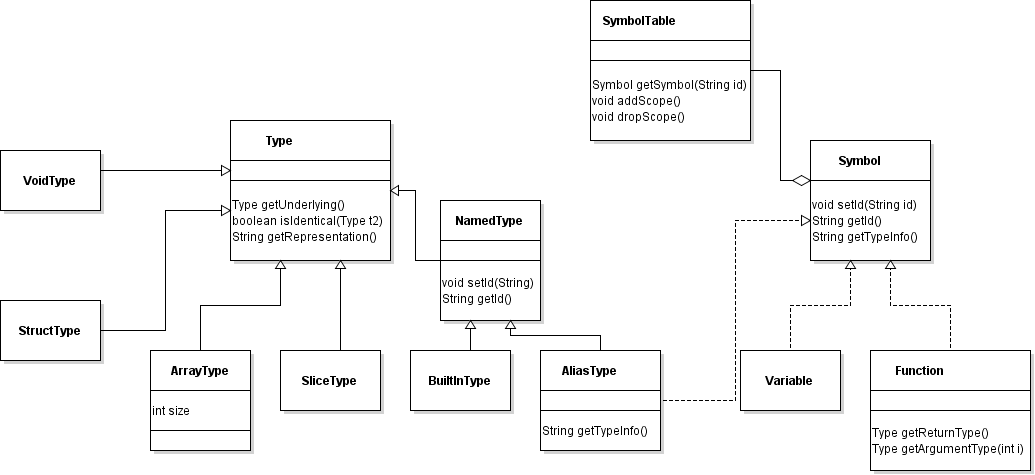
\includegraphics[width=\textwidth]{symbol_table_uml}
    \caption{Class hierarchy for GoLite types and symbols (property and method listings are non-exhaustive)}
    \label{fig:symbol_table_uml}
\end{figure}

These considerations led us to a number of particular decisions. First, we place functions outside the type hierarchy. While in Go functions are first class citizens, with their type given by the function signature, in GoLite they are not. Therefore, instead of implementing functions as instances of \texttt{Variable}, which would potentially allow them to be used where another objects of another type are required, we implemented a \texttt{Function} class which represents a particular function and stores both the function's identifier and its associated type information directly.

Second, we made \texttt{Symbol} an interface which is implemented by the \texttt{Variable}, \texttt{Function}, and \texttt{AliasType} classes. The difficulty here was that since \texttt{AliasType} is a subclass of \texttt{Type}, it could not also inherit from an abstract \texttt{Symbol} class. By making \texttt{Symbol} an interface, we allow \texttt{AliasType} instances into the symbol table directly without thereby making it possible to enter other types---for instance the \texttt{BuiltInType} which we use for \texttt{int}, \texttt{bool}, \texttt{alias}, and \texttt{rune}---illicitly. The downside of this design is that the \texttt{getId} and \texttt{setId} methods required by \texttt{Symbol} had to be implemented at least twice. However, this was sufficiently trivial that it did not change our decision. In fact, the duplication is so trivial that we did not even create a shared superclass for \texttt{Function} and \texttt{Variable} to reduce the duplication there.\footnote{We \emph{did}, however, create a \texttt{NamedType} class which is extended by both \texttt{BuiltInType} and \texttt{AliasType}. This class also implements the \texttt{isIdentical} and \texttt{getRepresentation} methods.}

A final decision worth noting is our use of the \texttt{VoidType} class. Since unfortunately Java does not make it possible to statically forbid null pointers, it is easy to introduce them accidentally. To help catch such cases, we use \texttt{VoidType} instead of \texttt{null} to represent the return type of a function that does not return a value.

\section{Pretty printers}
TODO

We extended the \verb|PrettyPrinter| class we implemented in Milestone 1 to have it print extra type information. By overriding the \verb|defaultOut| method, it was simple to have it look up and output the type of any node which is an instance of the \verb|PExp| (expression production) class as an inline comment.

\section{Code generation}
\subsection{Output considerations: JavaScript}
Transpiling to a higher level language like JavaScript entails different considerations than compiling to a lower-level language like C, or to bytecode or assembly language. Because JavaScript does not have static typing, it is possible to implement more flexible patterns, like functions which abstract over values of different types. But this flexibility comes at a cost, both in ensuring program correctness and in maintaining adequate performance. Short of syntax errors, flaws in the generated code will only ever be revealed when the code is run, rather than by the target-language compiler or a bytecode verifier. Similarly, unless performance is maintained as an explicit goal of code generation, it is very easy to generate output that is woefully inefficient---for instance, by delegating checks that could be done at compile time to runtime functions.

The strict mode introduced by the ECMAScript 5 standard helps somewhat to alleviate the correctness problem.\footnote{TODO cite} Code which requests strict mode opts in, in a backwards-compatible way, to slightly more stringent correctness checks. For instance, without strict mode assigning a value to an undeclared variable writes it to the global scope; with strict mode, this is an error. To move beyond what this could offer, we ran a suite of test programs through our compiler and compared the output to the Go source.

\subsection{Generation techniques}
Where possible, we made the ``obvious'' translation from GoLite to JavaScript. For many statements and expressions this was trivial. The control statements, for instance, were easily translated into JavaScript. However, we ran into a number of corner cases where the languages' semantics diverged. For instance, JavaScript does not do any kind of bounds checking for arrays***

TODO lvalues

We used JavaScript's objects---essentially mappings from strings to arbitrary values\footnote{We did not make any use of JavaScript's prototype system}---to implement structs. For both arrays and slices we used JavaScript's arrays, which are resizable and not inherently typed. JavaScript does not have pointers but instead implements both of these types as garbage-collected, pass-by-reference objects. This made them well suited to GoLite slices, but it was necessary to manually copy GoLite structs and arrays whenever they were reassigned to another value or passed to a function. ***

TODO call-site monomorphism

TODO scopes, alpha renaming

\subsection{Potential enhancements}
TODO typed arrays, source maps

\subsection{A translated program}
TODO

\section{Testing infrastructure}
We were provided with a wealth of test programs for the back end of the compiler; at present we have about 1000 programs in total. However, leveraging these programs effectively posed a challenge. We wanted to be able to run the whole suite in a tolerable time-frame and to extract meaningful information from the results, ideally without needing to alter or revize the majority of the programs or to manually examine their output.

In response, we developed a test running script, initially in Python. This script ran each of the programs and inferred the expected result from the program's path. For instance, \texttt{programs/invalid/parser/ trailing\_comma\_in\_print.go} should throw a parsing error. On the other hand, \texttt{programs/valid/teams/ parser/if\_else.go} (a test from another group) passes although it throws a type error, because it is only expected to be valid through the parsing stage. This was a sufficiently granular set of conditions to allow us to catch regressions, but it lacked flexibility. Some tests legitimately throw errors in a different stage that the one they test. For instance, some lexer tests only manifest in the parser. To handle these we wrote per-directory files called \texttt{test\_configuration.txt} which let us specify the expected error for a program without having to move it from the directory with the other programs that test the same issues.

The problem with this script is that it was too slow, because it called into \texttt{golite} in a subprocess for each file. (It also waited for each subprocess to exit, when they could have run in parallel.) We achieved huge performance improvements by rewriting the test runner as a JUnit test suite; this enabled it to use the GoLite code base directly, rather than as a separate subprocess, and also made it easier to more narrowly tailor what needed to run; whereas the Python test runner fully compiled the program, the JUnit tests only executed the compilation stages which were actually needed. (We could have done this using command-line options, but it would have taken more effort.) As a result of these advantages, the JUnit test runner tests the whole suite in less than five seconds.

However, we continued to maintain the Python implementation and expanded it with an interactive command-line interface to help administer the test suite. On encountering a failing test case, it gives the user options like editing the test case in Vim, changing what error is expected, writing a note about the program to file, reviewing the existing notes about the program, or ``tagging'' the program by writing to a file listing the test cases associated with a particular issue.

\subsection{Sample test session}
\begin{verbatim}
$ tools/run_test_programs.py -i programs/invalid --exclude programs/invalid/parsing/
TEST FAILED: programs/invalid/weeding/function_terminal_statement_is_for.go
   Expected weeding error but the test passed all stages
Response?
   c: continue      e: edit     q: quit
   s: set expected  r: rerun    ?: help
-> e
[opens in Vim]
-> note See if this case is supported by the spec
-> tag terminal_statements
-> continue
[...]
\end{verbatim}

\section{Conclusion}
TODO

\end{document}
